
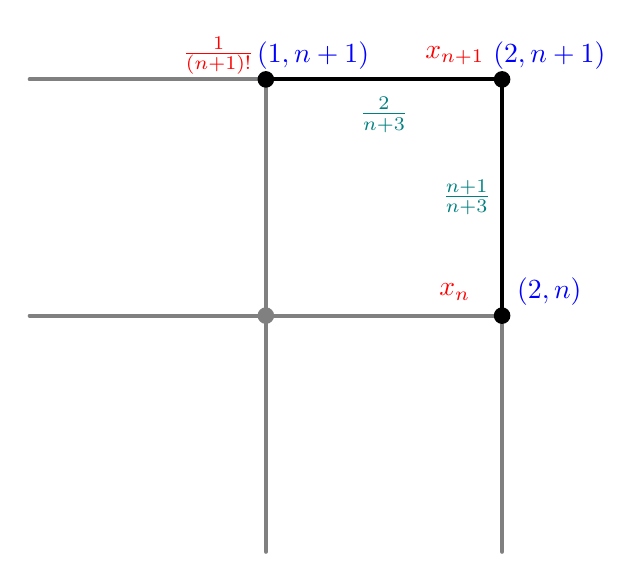
\begin{tikzpicture}[line cap=round,line join=round,x=3cm,y=3cm]


\draw[color=gray ,line width=0.5mm] (1,1) -- (0,1) node[sloped, pos=0.5, allow upside down]{\arrowIn}; 
\draw[color=gray ,line width=0.5mm] (2,1) -- (1,1) node[sloped, pos=0.5, allow upside down]{\arrowIn}; 
\draw[color=gray ,line width=0.5mm] (1,2) -- (0,2) node[sloped, pos=0.5, allow upside down]{\arrowIn}; 
\draw[color=black,line width=0.5mm] (2,2) -- (1,2) node[sloped, pos=0.5, allow upside down]{\arrowIn}; 
\draw[color=gray ,line width=0.5mm] (1,1) -- (1,0) node[sloped, pos=0.5, allow upside down]{\arrowIn}; 
\draw[color=gray ,line width=0.5mm] (1,2) -- (1,1) node[sloped, pos=0.5, allow upside down]{\arrowIn}; 
\draw[color=gray ,line width=0.5mm] (2,1) -- (2,0) node[sloped, pos=0.5, allow upside down]{\arrowIn}; 
\draw[color=black,line width=0.5mm] (2,2) -- (2,1) node[sloped, pos=0.5, allow upside down]{\arrowIn}; 

\fill[color=gray] (1,1) circle[radius=3pt];
\fill             (2,1) circle[radius=3pt];
\fill             (1,2) circle[radius=3pt];
\fill             (2,2) circle[radius=3pt];

\node[text=red] at ( 1.8, 1.1)  {$x_n$};
\node[text=red] at ( 0.8, 2.1)  {$\frac{1}{(n+1)!}$};
\node[text=red] at ( 1.8, 2.1)  {$x_{n+1}$};

\node[text=blue] at (2.2, 1.1)  {$(2,n)$};
\node[text=blue] at (1.2, 2.1)  {$(1,n+1)$};
\node[text=blue] at (2.2, 2.1)  {$(2,n+1)$};

\node[text=teal] at (1.5, 1.85)  {$\frac{2}{n+3}$};
\node[text=teal] at (1.85, 1.5)  {$\frac{n+1}{n+3}$};

\end{tikzpicture}
